\section{Evaluation}
\label{sec:evaluation}

\subsection{Storage Capacity}
\label{subsec:capacity}
\begin{figure}[t]
	\centering
	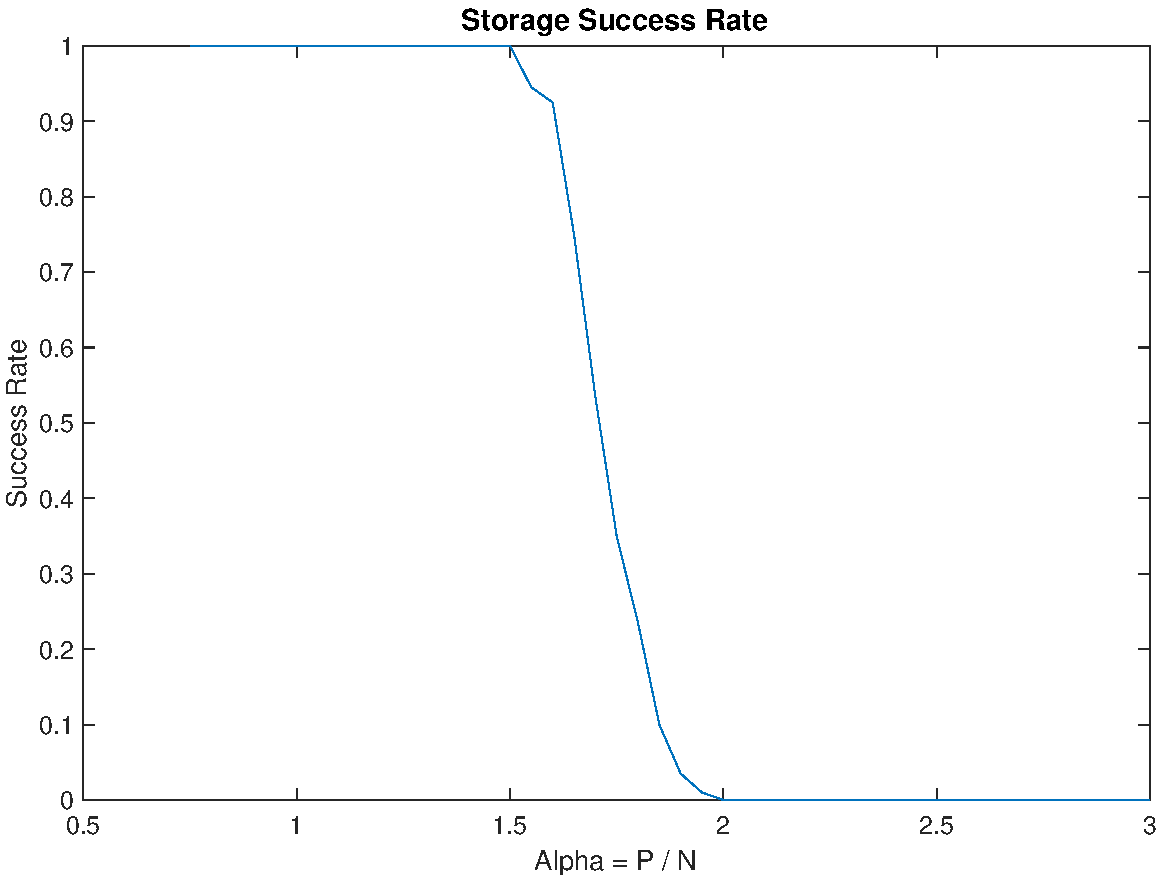
\includegraphics[width=\columnwidth]{figures/base}
    \caption{Storage success rate of a Rosenblatt perceptron as a function of $\alpha = P / N$. The experiments use $N = 500$, $n_{max} = 200$ and $n_D = 100$.}
	\label{fig:base}
\end{figure}

\cref{fig:base} shows the results of the base experiment using $N = 500$, $n_{max} = 200$ and $n_D = 100$.
The x-axis represent different values of $\alpha = P / N$, while the y-axis the success rate $Q_{l.s.}$.
As expected, the function looks like a step function from $1$ to $0$.
For $\alpha \approx 1.7$, the success rate $Q_{l.s.}$ drops from $1$ to $0$ very quickly. 

The value of $\alpha$ for which the function drops is called storage capacity of the perceptron.
For $N \to \infty$ (very large number of examples) and $n_{max} \to \infty$ (no limit on the maximum number of training epochs), the theoretical storage capacity of the Rosenblatt perceptron is $\alpha = 2$.

\subsection{Number of Epochs}
\label{subsec:epochs}
\begin{figure}[t]
	\centering
	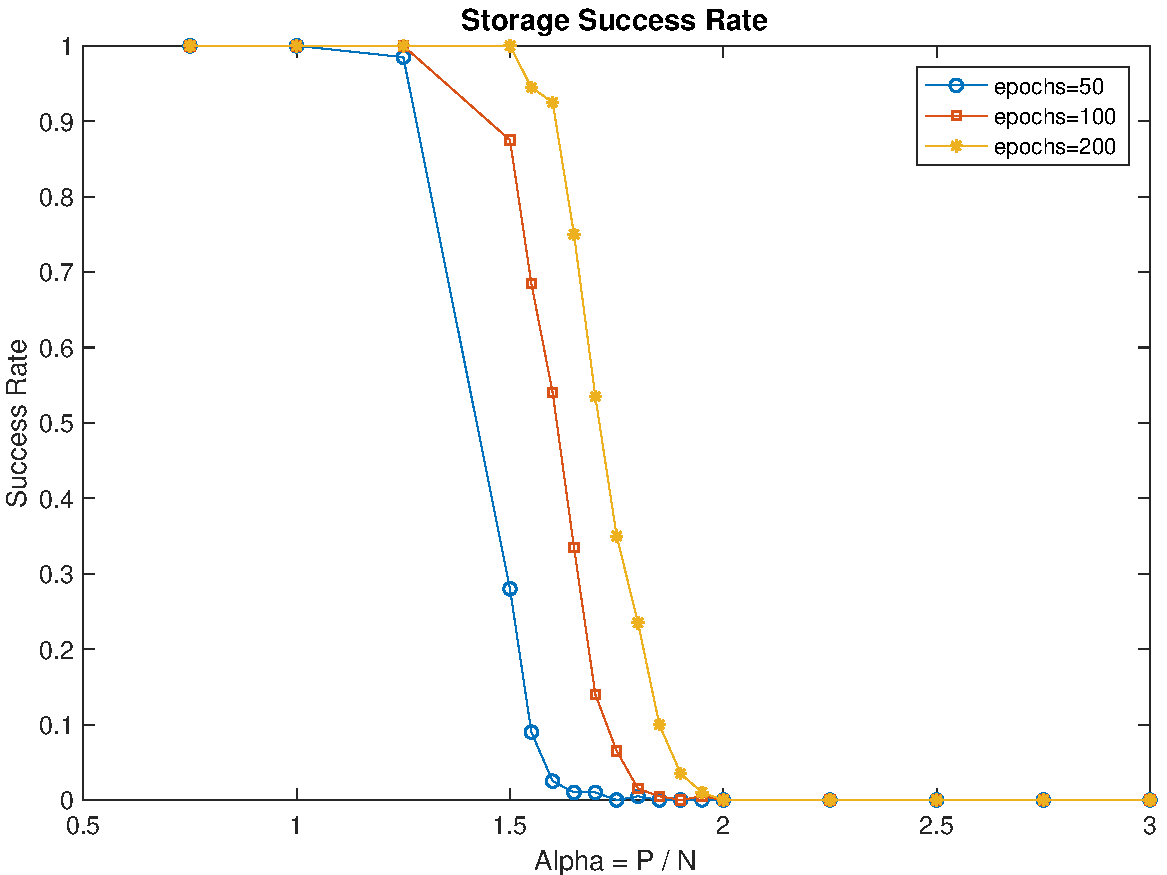
\includegraphics[width=\columnwidth]{figures/multiple_epochs}
    \caption{Storage success rate of a Rosenblatt perceptron as a function of $\alpha = P / N$ for different values of $n_{max}$.}
	\label{fig:multiple_epochs}
\end{figure}

The difference between the theoretical value and the experimental one are mainly due to the limited number of training epochs.
\cref{fig:multiple_epochs} gives an experimental proof of this statement:
for a very small number of epochs (eg. $n_{max} = 10$), the step is close to $\alpha = 1$, while for higher values of epochs the step moves closer and closer to the theoretical value $\alpha = 2$.

\subsection{Number of Dimensions}
\label{subsec:dimensions}
\begin{figure}[t]
	\centering
	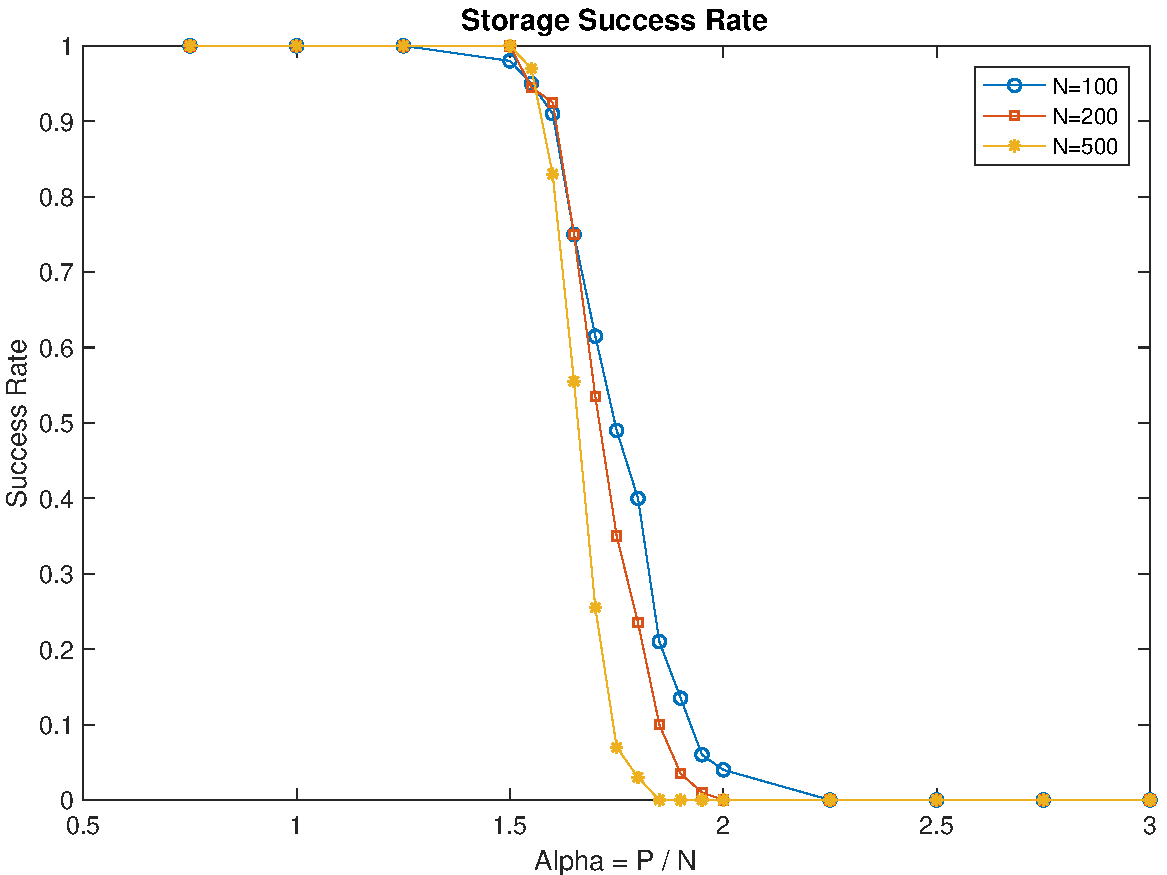
\includegraphics[width=\columnwidth]{figures/multiple_n}
    \caption{Storage success rate of a Rosenblatt perceptron as a function of $\alpha = P / N$ for different values of $N$.}
	\label{fig:multiple_n}
\end{figure}

The theoretical results are valid for $N \to \infty$.
However, real datasets have a limited number of features.
\cref{fig:multiple_n} shows the behaviour of the perceptron for different values of $N$.
For high values of $N$, the shape of the success rate $Q_{l.s.}$ as a function of $\alpha$ is similar to a step function.
For small values of $N$, the function looks like a smoothed step function:
the smaller $N$ is, the higher is the smoothing.

\subsection{Weight Update Criterion}
\label{subsec:c}
\begin{figure}[t]
	\centering
	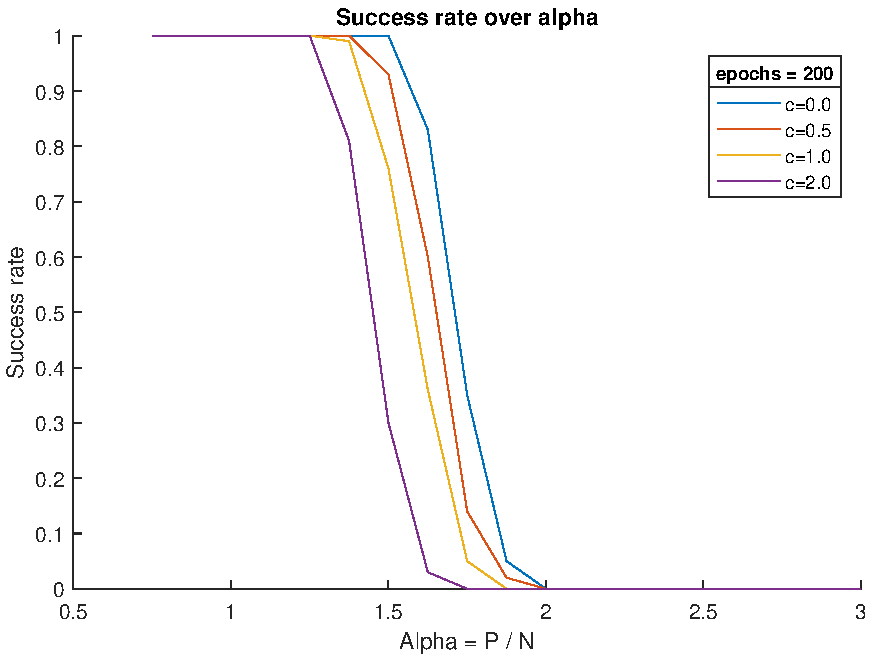
\includegraphics[width=\columnwidth]{figures/bonus_2_c}
    \caption{Storage success rate of a Rosenblatt perceptron as a function of $\alpha = P / N$ for different values of $c$.}
	\label{fig:multiple_c}
\end{figure}
The first experiment we ran to try to understand the contribute of the variable $c$ in the algorithm consisted in training the perceptron for different
values of it. As it is possible to notice in figure \ref{fig:multiple_c} the main effect is a shift to the left of the curve. This result was expected, because
$c$ introduces a step greater than zero in order to proceed to with the update of the weights's vector. What we thought is that if the value needed to perform
the update in greater also the number of epochs needed should be greater, proposing the hypothesis that $c$ works as a simple version of the learning rate that
we find in more complex neural networks.

\begin{figure}[t]
	\centering
	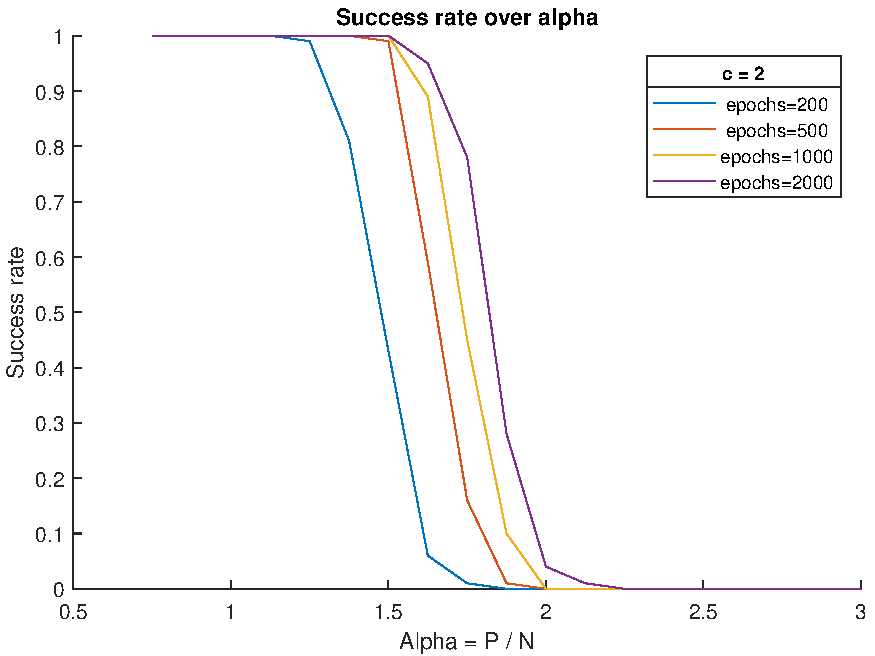
\includegraphics[width=\columnwidth]{figures/bonus_2_epoch}
    \caption{Storage success rate of a Rosenblatt perceptron as a function of $\alpha = P / N$ for different numbers of $epochs$ with fixed value of $c=2$.}
	\label{fig:fixed_c_multiple_epoch}
\end{figure}
For this reason we decided to simulate the behaviour of the curve for a given value of $c > 0$ and an increasing number of epochs. As it is possible to see
in figure \ref{fig:fixed_c_multiple_epoch} by increasing the number of epochs we \'pushed\' the curve toward the values that we got in the original experiment shown
in figure \ref{fig:base}, contrasting the effect of the increased value of $c$. The results we got from this experiment supported our hypothesis that $c$ behaves like
a learning rate. In fact the algorithm reaches almost the same results for different values of the variables and consistently modified number of epochs as reported in
figure \ref{fig:multiple_c_multiple_epoch}.

\begin{figure}[t]
	\centering
	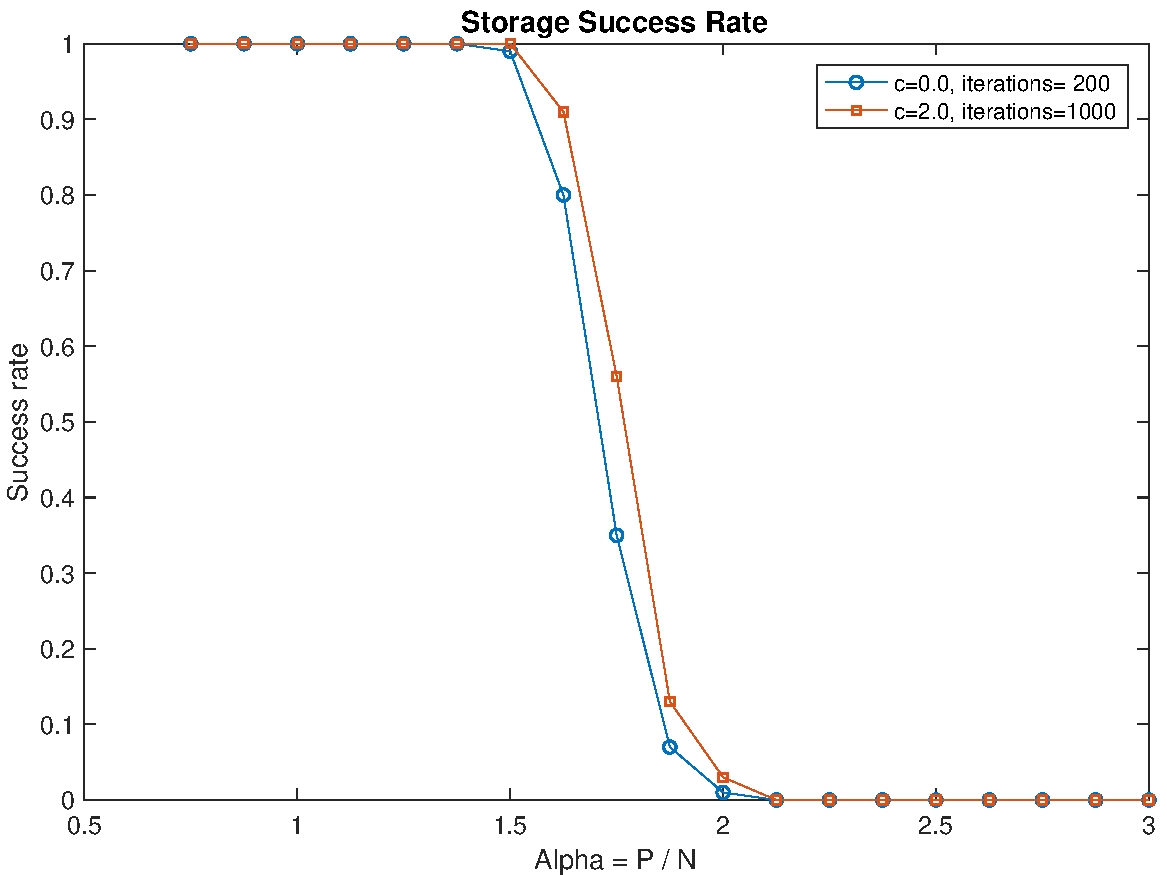
\includegraphics[width=\columnwidth]{figures/bonus_2_c_epoch}
    \caption{Storage success rate of a Rosenblatt perceptron as a function of $\alpha = P / N$ for different numbers of $epochs$ and $c$.}
	\label{fig:multiple_c_multiple_epoch}
\end{figure}

\subsection{Inhomogeneous Hyperplanes}
\label{subsec:homogeneous}
\begin{figure}[t]
	\centering
	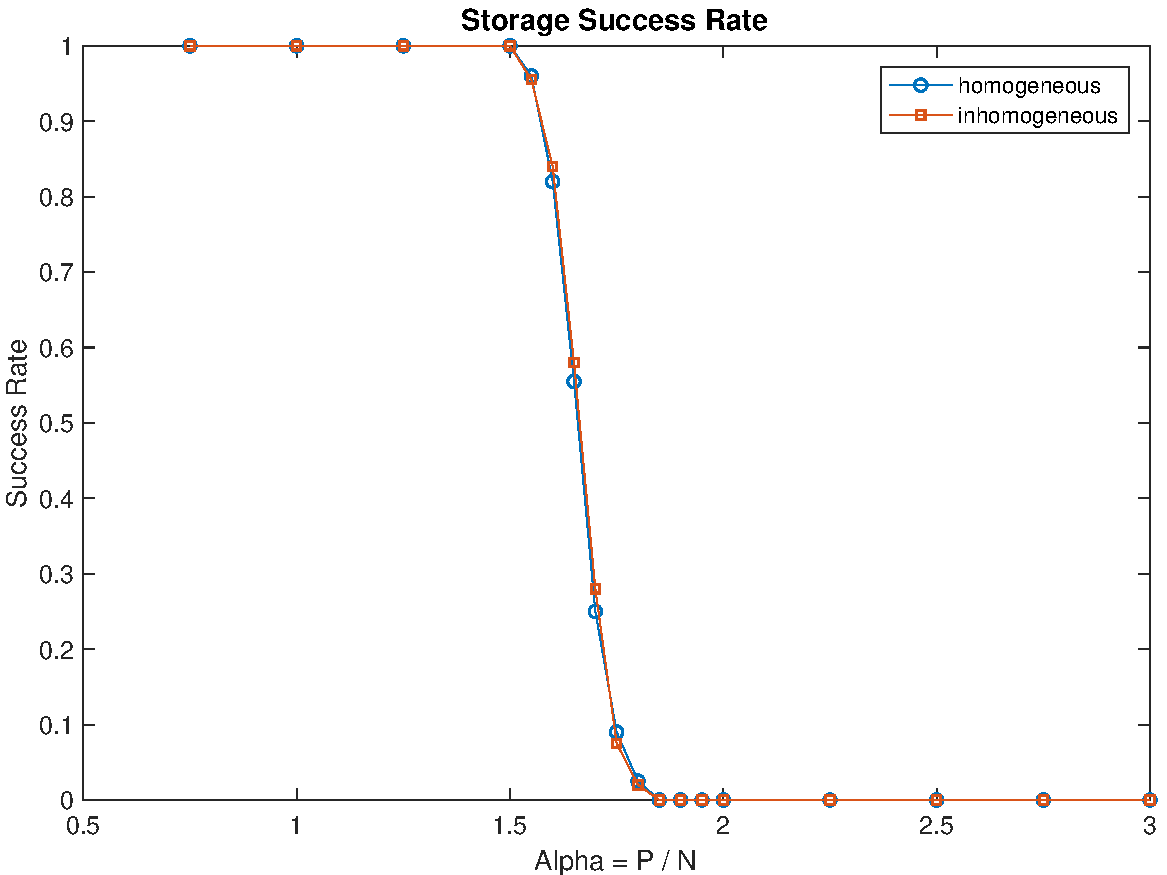
\includegraphics[width=\columnwidth]{figures/homogeneous}
    \caption{Storage success rate of a Rosenblatt perceptron and its inhomogeneous version as a function of $\alpha = P / N$.}
	\label{fig:homogeneous}
\end{figure}

We run an experiment to verify the behaviour of $Q_{l.s.}$ by allowing inhomogeneous hyperplanes:
we trained both a normal and modified perceptron on $200$ different datasets using $N = 500$, $n_max = 200$. 
\cref{fig:homogeneous} shows the results of the experiment.
As expected, the success rate $Q_{l.s.}$ of the inhomogeneous perceptron is slightly higher than homogeneous one.
However, the difference is not significant.

The problem of finding an inhomogeneously solution in $R^{N}$ can be solved by finding a homogeneously solution in $R^{N + 1}$.
In a second experiment, we compare the success rate $Q_{l.s.}$ of an inhomogeneous perceptron for $N = 500$ with an homogeneous perceptron for $N = 501$.
\cref{fig:homogeneous_n_n1} shows the result of this experiment.
As expected, the success rates for the $2$ perceptrons are very close to each other.

\begin{figure}[t]
	\centering
	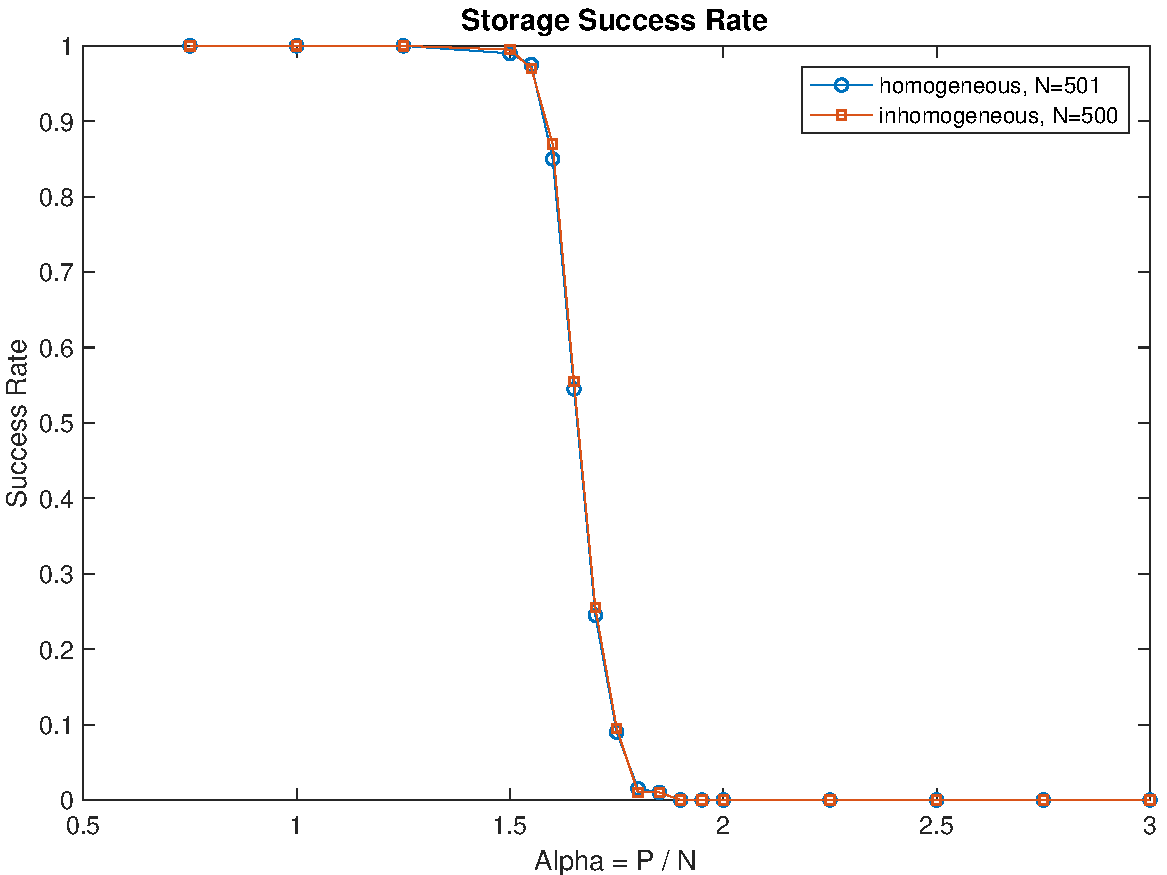
\includegraphics[width=\columnwidth]{figures/homogeneous_n_n1}
    \caption{Storage success rate of a homogeneous Rosenblatt perceptron with $N = 501$ and its inhomogeneous version with $N = 501$ as a function of $\alpha = P / N$.}
	\label{fig:homogeneous_n_n1}
\end{figure}
